% Created by tikzDevice version 0.12.6 on 2024-05-15 14:51:03
% !TEX encoding = UTF-8 Unicode
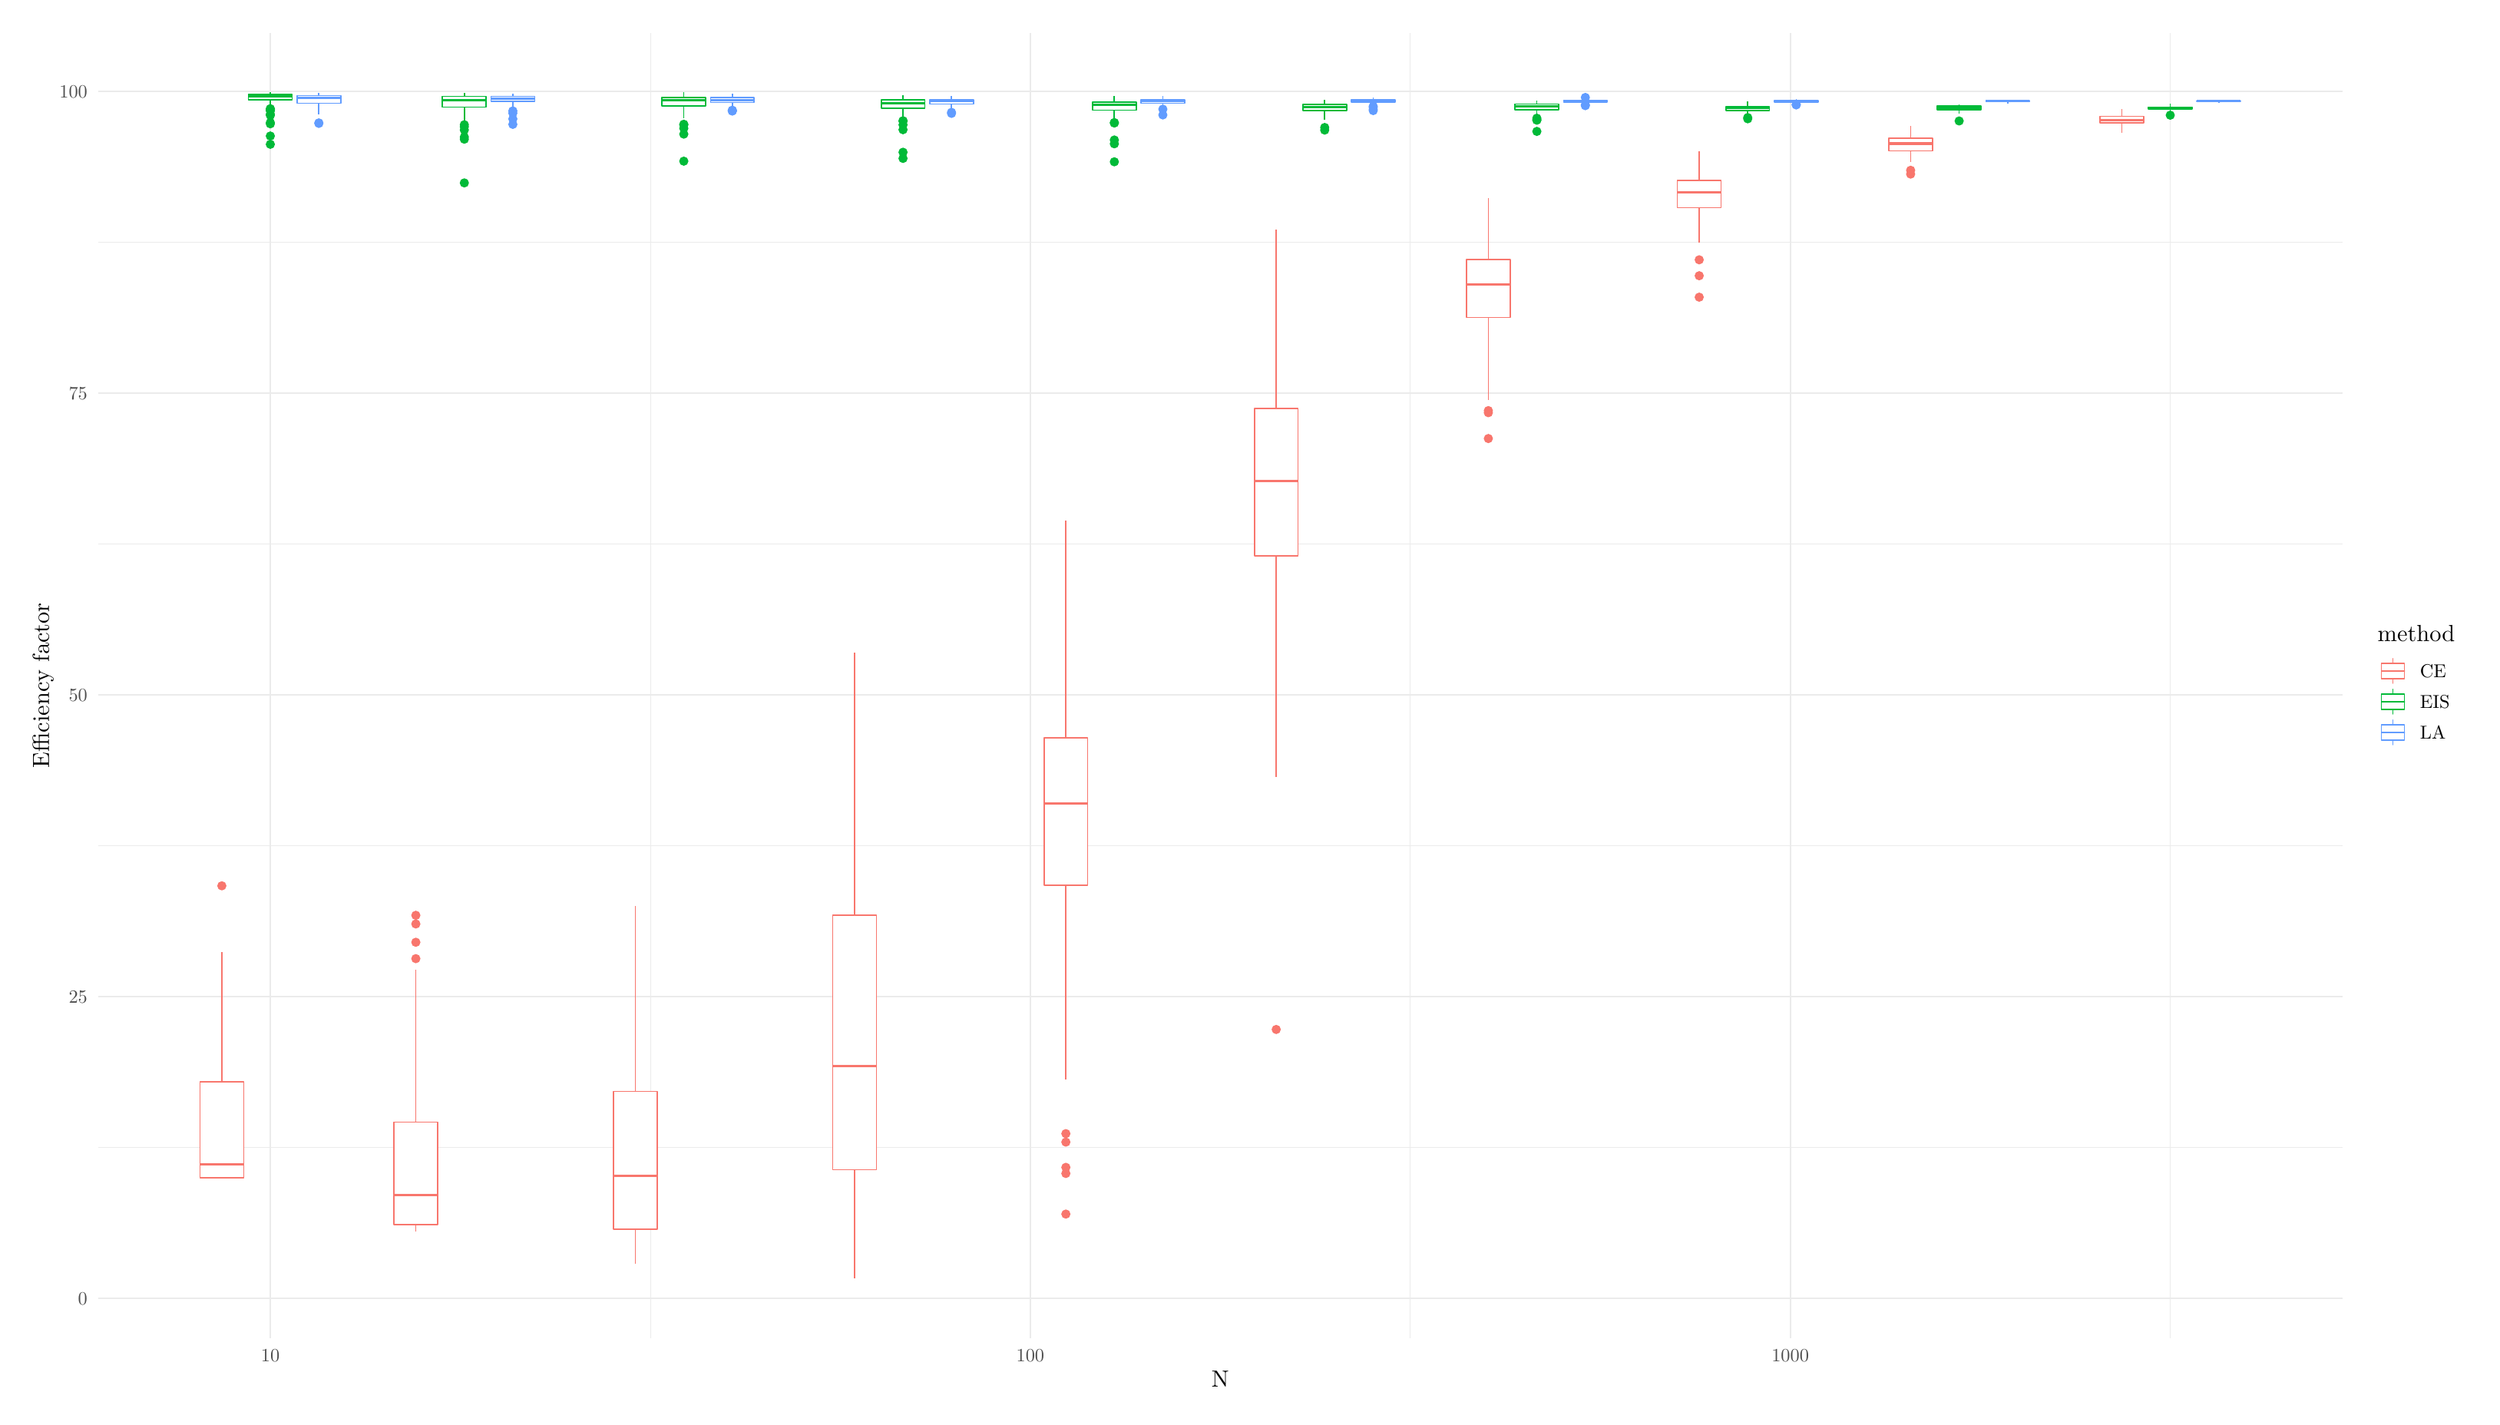
\begin{tikzpicture}[x=1pt,y=1pt]
\definecolor{fillColor}{RGB}{255,255,255}
\path[use as bounding box,fill=fillColor,fill opacity=0.00] (0,0) rectangle (1156.32,650.43);
\begin{scope}
\path[clip] ( 36.11, 30.69) rectangle (1092.47,644.93);
\definecolor{drawColor}{gray}{0.92}

\path[draw=drawColor,line width= 0.3pt,line join=round] ( 36.11,120.32) --
	(1092.47,120.32);

\path[draw=drawColor,line width= 0.3pt,line join=round] ( 36.11,262.33) --
	(1092.47,262.33);

\path[draw=drawColor,line width= 0.3pt,line join=round] ( 36.11,404.33) --
	(1092.47,404.33);

\path[draw=drawColor,line width= 0.3pt,line join=round] ( 36.11,546.33) --
	(1092.47,546.33);

\path[draw=drawColor,line width= 0.3pt,line join=round] (296.05, 30.69) --
	(296.05,644.93);

\path[draw=drawColor,line width= 0.3pt,line join=round] (653.71, 30.69) --
	(653.71,644.93);

\path[draw=drawColor,line width= 0.3pt,line join=round] (1011.37, 30.69) --
	(1011.37,644.93);

\path[draw=drawColor,line width= 0.6pt,line join=round] ( 36.11, 49.32) --
	(1092.47, 49.32);

\path[draw=drawColor,line width= 0.6pt,line join=round] ( 36.11,191.32) --
	(1092.47,191.32);

\path[draw=drawColor,line width= 0.6pt,line join=round] ( 36.11,333.33) --
	(1092.47,333.33);

\path[draw=drawColor,line width= 0.6pt,line join=round] ( 36.11,475.33) --
	(1092.47,475.33);

\path[draw=drawColor,line width= 0.6pt,line join=round] ( 36.11,617.34) --
	(1092.47,617.34);

\path[draw=drawColor,line width= 0.6pt,line join=round] (117.22, 30.69) --
	(117.22,644.93);

\path[draw=drawColor,line width= 0.6pt,line join=round] (474.88, 30.69) --
	(474.88,644.93);

\path[draw=drawColor,line width= 0.6pt,line join=round] (832.54, 30.69) --
	(832.54,644.93);
\definecolor{drawColor}{RGB}{248,118,109}
\definecolor{fillColor}{RGB}{248,118,109}

\path[draw=drawColor,line width= 0.4pt,line join=round,line cap=round,fill=fillColor] ( 94.40,243.52) circle (  1.96);

\path[draw=drawColor,line width= 0.6pt,line join=round] ( 94.40,151.32) -- ( 94.40,212.29);

\path[draw=drawColor,line width= 0.6pt,line join=round] ( 94.40,106.23) -- ( 94.40,106.12);
\definecolor{fillColor}{RGB}{255,255,255}

\path[draw=drawColor,line width= 0.6pt,line join=round,line cap=round,fill=fillColor] ( 84.13,151.32) --
	( 84.13,106.23) --
	(104.67,106.23) --
	(104.67,151.32) --
	( 84.13,151.32) --
	cycle;

\path[draw=drawColor,line width= 1.1pt,line join=round] ( 84.13,112.47) -- (104.67,112.47);
\definecolor{fillColor}{RGB}{248,118,109}

\path[draw=drawColor,line width= 0.4pt,line join=round,line cap=round,fill=fillColor] (185.70,209.25) circle (  1.96);

\path[draw=drawColor,line width= 0.4pt,line join=round,line cap=round,fill=fillColor] (185.70,229.64) circle (  1.96);

\path[draw=drawColor,line width= 0.4pt,line join=round,line cap=round,fill=fillColor] (185.70,216.96) circle (  1.96);

\path[draw=drawColor,line width= 0.4pt,line join=round,line cap=round,fill=fillColor] (185.70,225.58) circle (  1.96);

\path[draw=drawColor,line width= 0.6pt,line join=round] (185.70,132.33) -- (185.70,204.21);

\path[draw=drawColor,line width= 0.6pt,line join=round] (185.70, 84.17) -- (185.70, 80.88);
\definecolor{fillColor}{RGB}{255,255,255}

\path[draw=drawColor,line width= 0.6pt,line join=round,line cap=round,fill=fillColor] (175.43,132.33) --
	(175.43, 84.17) --
	(195.97, 84.17) --
	(195.97,132.33) --
	(175.43,132.33) --
	cycle;

\path[draw=drawColor,line width= 1.1pt,line join=round] (175.43, 98.15) -- (195.97, 98.15);

\path[draw=drawColor,line width= 0.6pt,line join=round] (288.99,146.81) -- (288.99,233.87);

\path[draw=drawColor,line width= 0.6pt,line join=round] (288.99, 81.98) -- (288.99, 65.55);

\path[draw=drawColor,line width= 0.6pt,line join=round,line cap=round,fill=fillColor] (278.72,146.81) --
	(278.72, 81.98) --
	(299.26, 81.98) --
	(299.26,146.81) --
	(278.72,146.81) --
	cycle;

\path[draw=drawColor,line width= 1.1pt,line join=round] (278.72,106.86) -- (299.26,106.86);

\path[draw=drawColor,line width= 0.6pt,line join=round] (392.15,229.71) -- (392.15,353.37);

\path[draw=drawColor,line width= 0.6pt,line join=round] (392.15,109.86) -- (392.15, 58.61);

\path[draw=drawColor,line width= 0.6pt,line join=round,line cap=round,fill=fillColor] (381.88,229.71) --
	(381.88,109.86) --
	(402.42,109.86) --
	(402.42,229.71) --
	(381.88,229.71) --
	cycle;

\path[draw=drawColor,line width= 1.1pt,line join=round] (381.88,158.81) -- (402.42,158.81);
\definecolor{fillColor}{RGB}{248,118,109}

\path[draw=drawColor,line width= 0.4pt,line join=round,line cap=round,fill=fillColor] (491.61,111.02) circle (  1.96);

\path[draw=drawColor,line width= 0.4pt,line join=round,line cap=round,fill=fillColor] (491.61, 89.03) circle (  1.96);

\path[draw=drawColor,line width= 0.4pt,line join=round,line cap=round,fill=fillColor] (491.61,126.90) circle (  1.96);

\path[draw=drawColor,line width= 0.4pt,line join=round,line cap=round,fill=fillColor] (491.61,108.14) circle (  1.96);

\path[draw=drawColor,line width= 0.4pt,line join=round,line cap=round,fill=fillColor] (491.61,122.91) circle (  1.96);

\path[draw=drawColor,line width= 0.6pt,line join=round] (491.61,313.28) -- (491.61,415.49);

\path[draw=drawColor,line width= 0.6pt,line join=round] (491.61,243.78) -- (491.61,152.38);
\definecolor{fillColor}{RGB}{255,255,255}

\path[draw=drawColor,line width= 0.6pt,line join=round,line cap=round,fill=fillColor] (481.34,313.28) --
	(481.34,243.78) --
	(501.88,243.78) --
	(501.88,313.28) --
	(481.34,313.28) --
	cycle;

\path[draw=drawColor,line width= 1.1pt,line join=round] (481.34,282.41) -- (501.88,282.41);
\definecolor{fillColor}{RGB}{248,118,109}

\path[draw=drawColor,line width= 0.4pt,line join=round,line cap=round,fill=fillColor] (590.61,175.92) circle (  1.96);

\path[draw=drawColor,line width= 0.6pt,line join=round] (590.61,468.08) -- (590.61,552.20);

\path[draw=drawColor,line width= 0.6pt,line join=round] (590.61,398.70) -- (590.61,294.91);
\definecolor{fillColor}{RGB}{255,255,255}

\path[draw=drawColor,line width= 0.6pt,line join=round,line cap=round,fill=fillColor] (580.34,468.08) --
	(580.34,398.70) --
	(600.88,398.70) --
	(600.88,468.08) --
	(580.34,468.08) --
	cycle;

\path[draw=drawColor,line width= 1.1pt,line join=round] (580.34,434.16) -- (600.88,434.16);
\definecolor{fillColor}{RGB}{248,118,109}

\path[draw=drawColor,line width= 0.4pt,line join=round,line cap=round,fill=fillColor] (690.44,454.03) circle (  1.96);

\path[draw=drawColor,line width= 0.4pt,line join=round,line cap=round,fill=fillColor] (690.44,466.19) circle (  1.96);

\path[draw=drawColor,line width= 0.4pt,line join=round,line cap=round,fill=fillColor] (690.44,467.17) circle (  1.96);

\path[draw=drawColor,line width= 0.6pt,line join=round] (690.44,538.19) -- (690.44,567.13);

\path[draw=drawColor,line width= 0.6pt,line join=round] (690.44,511.01) -- (690.44,472.25);
\definecolor{fillColor}{RGB}{255,255,255}

\path[draw=drawColor,line width= 0.6pt,line join=round,line cap=round,fill=fillColor] (680.17,538.19) --
	(680.17,511.01) --
	(700.71,511.01) --
	(700.71,538.19) --
	(680.17,538.19) --
	cycle;

\path[draw=drawColor,line width= 1.1pt,line join=round] (680.17,526.54) -- (700.71,526.54);
\definecolor{fillColor}{RGB}{248,118,109}

\path[draw=drawColor,line width= 0.4pt,line join=round,line cap=round,fill=fillColor] (789.68,538.15) circle (  1.96);

\path[draw=drawColor,line width= 0.4pt,line join=round,line cap=round,fill=fillColor] (789.68,530.65) circle (  1.96);

\path[draw=drawColor,line width= 0.4pt,line join=round,line cap=round,fill=fillColor] (789.68,520.56) circle (  1.96);

\path[draw=drawColor,line width= 0.6pt,line join=round] (789.68,575.49) -- (789.68,589.11);

\path[draw=drawColor,line width= 0.6pt,line join=round] (789.68,562.71) -- (789.68,546.38);
\definecolor{fillColor}{RGB}{255,255,255}

\path[draw=drawColor,line width= 0.6pt,line join=round,line cap=round,fill=fillColor] (779.41,575.49) --
	(779.41,562.71) --
	(799.95,562.71) --
	(799.95,575.49) --
	(779.41,575.49) --
	cycle;

\path[draw=drawColor,line width= 1.1pt,line join=round] (779.41,569.79) -- (799.95,569.79);
\definecolor{fillColor}{RGB}{248,118,109}

\path[draw=drawColor,line width= 0.4pt,line join=round,line cap=round,fill=fillColor] (889.18,578.48) circle (  1.96);

\path[draw=drawColor,line width= 0.4pt,line join=round,line cap=round,fill=fillColor] (889.18,580.28) circle (  1.96);

\path[draw=drawColor,line width= 0.6pt,line join=round] (889.18,595.39) -- (889.18,601.30);

\path[draw=drawColor,line width= 0.6pt,line join=round] (889.18,589.46) -- (889.18,584.08);
\definecolor{fillColor}{RGB}{255,255,255}

\path[draw=drawColor,line width= 0.6pt,line join=round,line cap=round,fill=fillColor] (878.91,595.39) --
	(878.91,589.46) --
	(899.46,589.46) --
	(899.46,595.39) --
	(878.91,595.39) --
	cycle;

\path[draw=drawColor,line width= 1.1pt,line join=round] (878.91,592.85) -- (899.46,592.85);

\path[draw=drawColor,line width= 0.6pt,line join=round] (988.53,605.72) -- (988.53,609.07);

\path[draw=drawColor,line width= 0.6pt,line join=round] (988.53,602.54) -- (988.53,598.02);

\path[draw=drawColor,line width= 0.6pt,line join=round,line cap=round,fill=fillColor] (978.26,605.72) --
	(978.26,602.54) --
	(998.80,602.54) --
	(998.80,605.72) --
	(978.26,605.72) --
	cycle;

\path[draw=drawColor,line width= 1.1pt,line join=round] (978.26,604.03) -- (998.80,604.03);
\definecolor{drawColor}{RGB}{0,186,56}
\definecolor{fillColor}{RGB}{0,186,56}

\path[draw=drawColor,line width= 0.4pt,line join=round,line cap=round,fill=fillColor] (117.22,606.65) circle (  1.96);

\path[draw=drawColor,line width= 0.4pt,line join=round,line cap=round,fill=fillColor] (117.22,592.51) circle (  1.96);

\path[draw=drawColor,line width= 0.4pt,line join=round,line cap=round,fill=fillColor] (117.22,602.15) circle (  1.96);

\path[draw=drawColor,line width= 0.4pt,line join=round,line cap=round,fill=fillColor] (117.22,608.67) circle (  1.96);

\path[draw=drawColor,line width= 0.4pt,line join=round,line cap=round,fill=fillColor] (117.22,608.99) circle (  1.96);

\path[draw=drawColor,line width= 0.4pt,line join=round,line cap=round,fill=fillColor] (117.22,608.76) circle (  1.96);

\path[draw=drawColor,line width= 0.4pt,line join=round,line cap=round,fill=fillColor] (117.22,596.41) circle (  1.96);

\path[draw=drawColor,line width= 0.4pt,line join=round,line cap=round,fill=fillColor] (117.22,606.16) circle (  1.96);

\path[draw=drawColor,line width= 0.4pt,line join=round,line cap=round,fill=fillColor] (117.22,608.28) circle (  1.96);

\path[draw=drawColor,line width= 0.4pt,line join=round,line cap=round,fill=fillColor] (117.22,602.70) circle (  1.96);

\path[draw=drawColor,line width= 0.4pt,line join=round,line cap=round,fill=fillColor] (117.22,609.27) circle (  1.96);

\path[draw=drawColor,line width= 0.6pt,line join=round] (117.22,616.06) -- (117.22,617.01);

\path[draw=drawColor,line width= 0.6pt,line join=round] (117.22,613.56) -- (117.22,610.21);
\definecolor{fillColor}{RGB}{255,255,255}

\path[draw=drawColor,line width= 0.6pt,line join=round,line cap=round,fill=fillColor] (106.95,616.06) --
	(106.95,613.56) --
	(127.49,613.56) --
	(127.49,616.06) --
	(106.95,616.06) --
	cycle;

\path[draw=drawColor,line width= 1.1pt,line join=round] (106.95,614.97) -- (127.49,614.97);
\definecolor{fillColor}{RGB}{0,186,56}

\path[draw=drawColor,line width= 0.4pt,line join=round,line cap=round,fill=fillColor] (208.52,594.91) circle (  1.96);

\path[draw=drawColor,line width= 0.4pt,line join=round,line cap=round,fill=fillColor] (208.52,595.93) circle (  1.96);

\path[draw=drawColor,line width= 0.4pt,line join=round,line cap=round,fill=fillColor] (208.52,601.72) circle (  1.96);

\path[draw=drawColor,line width= 0.4pt,line join=round,line cap=round,fill=fillColor] (208.52,574.34) circle (  1.96);

\path[draw=drawColor,line width= 0.4pt,line join=round,line cap=round,fill=fillColor] (208.52,599.26) circle (  1.96);

\path[draw=drawColor,line width= 0.4pt,line join=round,line cap=round,fill=fillColor] (208.52,600.76) circle (  1.96);

\path[draw=drawColor,line width= 0.6pt,line join=round] (208.52,615.11) -- (208.52,616.82);

\path[draw=drawColor,line width= 0.6pt,line join=round] (208.52,610.06) -- (208.52,602.95);
\definecolor{fillColor}{RGB}{255,255,255}

\path[draw=drawColor,line width= 0.6pt,line join=round,line cap=round,fill=fillColor] (198.25,615.11) --
	(198.25,610.06) --
	(218.80,610.06) --
	(218.80,615.11) --
	(198.25,615.11) --
	cycle;

\path[draw=drawColor,line width= 1.1pt,line join=round] (198.25,613.39) -- (218.80,613.39);
\definecolor{fillColor}{RGB}{0,186,56}

\path[draw=drawColor,line width= 0.4pt,line join=round,line cap=round,fill=fillColor] (311.81,597.30) circle (  1.96);

\path[draw=drawColor,line width= 0.4pt,line join=round,line cap=round,fill=fillColor] (311.81,601.65) circle (  1.96);

\path[draw=drawColor,line width= 0.4pt,line join=round,line cap=round,fill=fillColor] (311.81,601.94) circle (  1.96);

\path[draw=drawColor,line width= 0.4pt,line join=round,line cap=round,fill=fillColor] (311.81,584.57) circle (  1.96);

\path[draw=drawColor,line width= 0.4pt,line join=round,line cap=round,fill=fillColor] (311.81,600.02) circle (  1.96);

\path[draw=drawColor,line width= 0.6pt,line join=round] (311.81,614.47) -- (311.81,616.94);

\path[draw=drawColor,line width= 0.6pt,line join=round] (311.81,610.54) -- (311.81,604.88);
\definecolor{fillColor}{RGB}{255,255,255}

\path[draw=drawColor,line width= 0.6pt,line join=round,line cap=round,fill=fillColor] (301.54,614.47) --
	(301.54,610.54) --
	(322.09,610.54) --
	(322.09,614.47) --
	(301.54,614.47) --
	cycle;

\path[draw=drawColor,line width= 1.1pt,line join=round] (301.54,613.13) -- (322.09,613.13);
\definecolor{fillColor}{RGB}{0,186,56}

\path[draw=drawColor,line width= 0.4pt,line join=round,line cap=round,fill=fillColor] (414.98,601.68) circle (  1.96);

\path[draw=drawColor,line width= 0.4pt,line join=round,line cap=round,fill=fillColor] (414.98,588.77) circle (  1.96);

\path[draw=drawColor,line width= 0.4pt,line join=round,line cap=round,fill=fillColor] (414.98,603.40) circle (  1.96);

\path[draw=drawColor,line width= 0.4pt,line join=round,line cap=round,fill=fillColor] (414.98,603.59) circle (  1.96);

\path[draw=drawColor,line width= 0.4pt,line join=round,line cap=round,fill=fillColor] (414.98,599.39) circle (  1.96);

\path[draw=drawColor,line width= 0.4pt,line join=round,line cap=round,fill=fillColor] (414.98,585.87) circle (  1.96);

\path[draw=drawColor,line width= 0.6pt,line join=round] (414.98,613.47) -- (414.98,615.44);

\path[draw=drawColor,line width= 0.6pt,line join=round] (414.98,609.57) -- (414.98,603.74);
\definecolor{fillColor}{RGB}{255,255,255}

\path[draw=drawColor,line width= 0.6pt,line join=round,line cap=round,fill=fillColor] (404.71,613.47) --
	(404.71,609.57) --
	(425.25,609.57) --
	(425.25,613.47) --
	(404.71,613.47) --
	cycle;

\path[draw=drawColor,line width= 1.1pt,line join=round] (404.71,611.68) -- (425.25,611.68);
\definecolor{fillColor}{RGB}{0,186,56}

\path[draw=drawColor,line width= 0.4pt,line join=round,line cap=round,fill=fillColor] (514.43,594.54) circle (  1.96);

\path[draw=drawColor,line width= 0.4pt,line join=round,line cap=round,fill=fillColor] (514.43,602.74) circle (  1.96);

\path[draw=drawColor,line width= 0.4pt,line join=round,line cap=round,fill=fillColor] (514.43,592.74) circle (  1.96);

\path[draw=drawColor,line width= 0.4pt,line join=round,line cap=round,fill=fillColor] (514.43,584.27) circle (  1.96);

\path[draw=drawColor,line width= 0.4pt,line join=round,line cap=round,fill=fillColor] (514.43,602.51) circle (  1.96);

\path[draw=drawColor,line width= 0.6pt,line join=round] (514.43,612.42) -- (514.43,615.14);

\path[draw=drawColor,line width= 0.6pt,line join=round] (514.43,608.60) -- (514.43,603.39);
\definecolor{fillColor}{RGB}{255,255,255}

\path[draw=drawColor,line width= 0.6pt,line join=round,line cap=round,fill=fillColor] (504.16,612.42) --
	(504.16,608.60) --
	(524.71,608.60) --
	(524.71,612.42) --
	(504.16,612.42) --
	cycle;

\path[draw=drawColor,line width= 1.1pt,line join=round] (504.16,611.06) -- (524.71,611.06);
\definecolor{fillColor}{RGB}{0,186,56}

\path[draw=drawColor,line width= 0.4pt,line join=round,line cap=round,fill=fillColor] (613.43,600.42) circle (  1.96);

\path[draw=drawColor,line width= 0.4pt,line join=round,line cap=round,fill=fillColor] (613.43,599.20) circle (  1.96);

\path[draw=drawColor,line width= 0.6pt,line join=round] (613.43,611.39) -- (613.43,613.55);

\path[draw=drawColor,line width= 0.6pt,line join=round] (613.43,608.29) -- (613.43,603.90);
\definecolor{fillColor}{RGB}{255,255,255}

\path[draw=drawColor,line width= 0.6pt,line join=round,line cap=round,fill=fillColor] (603.16,611.39) --
	(603.16,608.29) --
	(623.71,608.29) --
	(623.71,611.39) --
	(603.16,611.39) --
	cycle;

\path[draw=drawColor,line width= 1.1pt,line join=round] (603.16,610.12) -- (623.71,610.12);
\definecolor{fillColor}{RGB}{0,186,56}

\path[draw=drawColor,line width= 0.4pt,line join=round,line cap=round,fill=fillColor] (713.27,604.00) circle (  1.96);

\path[draw=drawColor,line width= 0.4pt,line join=round,line cap=round,fill=fillColor] (713.27,604.79) circle (  1.96);

\path[draw=drawColor,line width= 0.4pt,line join=round,line cap=round,fill=fillColor] (713.27,598.58) circle (  1.96);

\path[draw=drawColor,line width= 0.4pt,line join=round,line cap=round,fill=fillColor] (713.27,603.87) circle (  1.96);

\path[draw=drawColor,line width= 0.6pt,line join=round] (713.27,611.48) -- (713.27,612.95);

\path[draw=drawColor,line width= 0.6pt,line join=round] (713.27,608.82) -- (713.27,605.17);
\definecolor{fillColor}{RGB}{255,255,255}

\path[draw=drawColor,line width= 0.6pt,line join=round,line cap=round,fill=fillColor] (703.00,611.48) --
	(703.00,608.82) --
	(723.54,608.82) --
	(723.54,611.48) --
	(703.00,611.48) --
	cycle;

\path[draw=drawColor,line width= 1.1pt,line join=round] (703.00,610.23) -- (723.54,610.23);
\definecolor{fillColor}{RGB}{0,186,56}

\path[draw=drawColor,line width= 0.4pt,line join=round,line cap=round,fill=fillColor] (812.51,604.51) circle (  1.96);

\path[draw=drawColor,line width= 0.4pt,line join=round,line cap=round,fill=fillColor] (812.51,605.09) circle (  1.96);

\path[draw=drawColor,line width= 0.6pt,line join=round] (812.51,610.23) -- (812.51,612.69);

\path[draw=drawColor,line width= 0.6pt,line join=round] (812.51,608.44) -- (812.51,606.21);
\definecolor{fillColor}{RGB}{255,255,255}

\path[draw=drawColor,line width= 0.6pt,line join=round,line cap=round,fill=fillColor] (802.24,610.23) --
	(802.24,608.44) --
	(822.78,608.44) --
	(822.78,610.23) --
	(802.24,610.23) --
	cycle;

\path[draw=drawColor,line width= 1.1pt,line join=round] (802.24,609.58) -- (822.78,609.58);
\definecolor{fillColor}{RGB}{0,186,56}

\path[draw=drawColor,line width= 0.4pt,line join=round,line cap=round,fill=fillColor] (912.01,603.49) circle (  1.96);

\path[draw=drawColor,line width= 0.6pt,line join=round] (912.01,610.46) -- (912.01,611.36);

\path[draw=drawColor,line width= 0.6pt,line join=round] (912.01,608.86) -- (912.01,606.91);
\definecolor{fillColor}{RGB}{255,255,255}

\path[draw=drawColor,line width= 0.6pt,line join=round,line cap=round,fill=fillColor] (901.74,610.46) --
	(901.74,608.86) --
	(922.28,608.86) --
	(922.28,610.46) --
	(901.74,610.46) --
	cycle;

\path[draw=drawColor,line width= 1.1pt,line join=round] (901.74,609.58) -- (922.28,609.58);
\definecolor{fillColor}{RGB}{0,186,56}

\path[draw=drawColor,line width= 0.4pt,line join=round,line cap=round,fill=fillColor] (1011.36,606.21) circle (  1.96);

\path[draw=drawColor,line width= 0.6pt,line join=round] (1011.36,610.06) -- (1011.36,611.59);

\path[draw=drawColor,line width= 0.6pt,line join=round] (1011.36,609.03) -- (1011.36,607.80);
\definecolor{fillColor}{RGB}{255,255,255}

\path[draw=drawColor,line width= 0.6pt,line join=round,line cap=round,fill=fillColor] (1001.08,610.06) --
	(1001.08,609.03) --
	(1021.63,609.03) --
	(1021.63,610.06) --
	(1001.08,610.06) --
	cycle;

\path[draw=drawColor,line width= 1.1pt,line join=round] (1001.08,609.56) -- (1021.63,609.56);
\definecolor{drawColor}{RGB}{97,156,255}
\definecolor{fillColor}{RGB}{97,156,255}

\path[draw=drawColor,line width= 0.4pt,line join=round,line cap=round,fill=fillColor] (140.05,602.35) circle (  1.96);

\path[draw=drawColor,line width= 0.4pt,line join=round,line cap=round,fill=fillColor] (140.05,602.58) circle (  1.96);

\path[draw=drawColor,line width= 0.6pt,line join=round] (140.05,615.40) -- (140.05,616.78);

\path[draw=drawColor,line width= 0.6pt,line join=round] (140.05,611.77) -- (140.05,606.51);
\definecolor{fillColor}{RGB}{255,255,255}

\path[draw=drawColor,line width= 0.6pt,line join=round,line cap=round,fill=fillColor] (129.78,615.40) --
	(129.78,611.77) --
	(150.32,611.77) --
	(150.32,615.40) --
	(129.78,615.40) --
	cycle;

\path[draw=drawColor,line width= 1.1pt,line join=round] (129.78,614.29) -- (150.32,614.29);
\definecolor{fillColor}{RGB}{97,156,255}

\path[draw=drawColor,line width= 0.4pt,line join=round,line cap=round,fill=fillColor] (231.35,601.89) circle (  1.96);

\path[draw=drawColor,line width= 0.4pt,line join=round,line cap=round,fill=fillColor] (231.35,604.45) circle (  1.96);

\path[draw=drawColor,line width= 0.4pt,line join=round,line cap=round,fill=fillColor] (231.35,607.16) circle (  1.96);

\path[draw=drawColor,line width= 0.4pt,line join=round,line cap=round,fill=fillColor] (231.35,608.22) circle (  1.96);

\path[draw=drawColor,line width= 0.6pt,line join=round] (231.35,615.11) -- (231.35,616.51);

\path[draw=drawColor,line width= 0.6pt,line join=round] (231.35,612.63) -- (231.35,608.92);
\definecolor{fillColor}{RGB}{255,255,255}

\path[draw=drawColor,line width= 0.6pt,line join=round,line cap=round,fill=fillColor] (221.08,615.11) --
	(221.08,612.63) --
	(241.62,612.63) --
	(241.62,615.11) --
	(221.08,615.11) --
	cycle;

\path[draw=drawColor,line width= 1.1pt,line join=round] (221.08,613.88) -- (241.62,613.88);
\definecolor{fillColor}{RGB}{97,156,255}

\path[draw=drawColor,line width= 0.4pt,line join=round,line cap=round,fill=fillColor] (334.64,608.19) circle (  1.96);

\path[draw=drawColor,line width= 0.4pt,line join=round,line cap=round,fill=fillColor] (334.64,608.55) circle (  1.96);

\path[draw=drawColor,line width= 0.4pt,line join=round,line cap=round,fill=fillColor] (334.64,608.20) circle (  1.96);

\path[draw=drawColor,line width= 0.4pt,line join=round,line cap=round,fill=fillColor] (334.64,608.38) circle (  1.96);

\path[draw=drawColor,line width= 0.6pt,line join=round] (334.64,614.47) -- (334.64,616.19);

\path[draw=drawColor,line width= 0.6pt,line join=round] (334.64,612.21) -- (334.64,610.14);
\definecolor{fillColor}{RGB}{255,255,255}

\path[draw=drawColor,line width= 0.6pt,line join=round,line cap=round,fill=fillColor] (324.37,614.47) --
	(324.37,612.21) --
	(344.91,612.21) --
	(344.91,614.47) --
	(324.37,614.47) --
	cycle;

\path[draw=drawColor,line width= 1.1pt,line join=round] (324.37,613.25) -- (344.91,613.25);
\definecolor{fillColor}{RGB}{97,156,255}

\path[draw=drawColor,line width= 0.4pt,line join=round,line cap=round,fill=fillColor] (437.80,607.54) circle (  1.96);

\path[draw=drawColor,line width= 0.4pt,line join=round,line cap=round,fill=fillColor] (437.80,607.06) circle (  1.96);

\path[draw=drawColor,line width= 0.6pt,line join=round] (437.80,613.53) -- (437.80,615.41);

\path[draw=drawColor,line width= 0.6pt,line join=round] (437.80,611.40) -- (437.80,608.95);
\definecolor{fillColor}{RGB}{255,255,255}

\path[draw=drawColor,line width= 0.6pt,line join=round,line cap=round,fill=fillColor] (427.53,613.53) --
	(427.53,611.40) --
	(448.07,611.40) --
	(448.07,613.53) --
	(427.53,613.53) --
	cycle;

\path[draw=drawColor,line width= 1.1pt,line join=round] (427.53,612.88) -- (448.07,612.88);
\definecolor{fillColor}{RGB}{97,156,255}

\path[draw=drawColor,line width= 0.4pt,line join=round,line cap=round,fill=fillColor] (537.26,606.33) circle (  1.96);

\path[draw=drawColor,line width= 0.4pt,line join=round,line cap=round,fill=fillColor] (537.26,609.03) circle (  1.96);

\path[draw=drawColor,line width= 0.6pt,line join=round] (537.26,613.54) -- (537.26,615.31);

\path[draw=drawColor,line width= 0.6pt,line join=round] (537.26,611.88) -- (537.26,609.72);
\definecolor{fillColor}{RGB}{255,255,255}

\path[draw=drawColor,line width= 0.6pt,line join=round,line cap=round,fill=fillColor] (526.99,613.54) --
	(526.99,611.88) --
	(547.53,611.88) --
	(547.53,613.54) --
	(526.99,613.54) --
	cycle;

\path[draw=drawColor,line width= 1.1pt,line join=round] (526.99,612.82) -- (547.53,612.82);
\definecolor{fillColor}{RGB}{97,156,255}

\path[draw=drawColor,line width= 0.4pt,line join=round,line cap=round,fill=fillColor] (636.26,608.38) circle (  1.96);

\path[draw=drawColor,line width= 0.4pt,line join=round,line cap=round,fill=fillColor] (636.26,608.94) circle (  1.96);

\path[draw=drawColor,line width= 0.4pt,line join=round,line cap=round,fill=fillColor] (636.26,610.38) circle (  1.96);

\path[draw=drawColor,line width= 0.4pt,line join=round,line cap=round,fill=fillColor] (636.26,609.99) circle (  1.96);

\path[draw=drawColor,line width= 0.6pt,line join=round] (636.26,613.46) -- (636.26,614.64);

\path[draw=drawColor,line width= 0.6pt,line join=round] (636.26,612.25) -- (636.26,611.08);
\definecolor{fillColor}{RGB}{255,255,255}

\path[draw=drawColor,line width= 0.6pt,line join=round,line cap=round,fill=fillColor] (625.99,613.46) --
	(625.99,612.25) --
	(646.53,612.25) --
	(646.53,613.46) --
	(625.99,613.46) --
	cycle;

\path[draw=drawColor,line width= 1.1pt,line join=round] (625.99,613.01) -- (646.53,613.01);
\definecolor{fillColor}{RGB}{97,156,255}

\path[draw=drawColor,line width= 0.4pt,line join=round,line cap=round,fill=fillColor] (736.09,610.70) circle (  1.96);

\path[draw=drawColor,line width= 0.4pt,line join=round,line cap=round,fill=fillColor] (736.09,611.05) circle (  1.96);

\path[draw=drawColor,line width= 0.4pt,line join=round,line cap=round,fill=fillColor] (736.09,614.55) circle (  1.96);

\path[draw=drawColor,line width= 0.6pt,line join=round] (736.09,613.21) -- (736.09,614.04);

\path[draw=drawColor,line width= 0.6pt,line join=round] (736.09,612.45) -- (736.09,611.38);
\definecolor{fillColor}{RGB}{255,255,255}

\path[draw=drawColor,line width= 0.6pt,line join=round,line cap=round,fill=fillColor] (725.82,613.21) --
	(725.82,612.45) --
	(746.36,612.45) --
	(746.36,613.21) --
	(725.82,613.21) --
	cycle;

\path[draw=drawColor,line width= 1.1pt,line join=round] (725.82,612.90) -- (746.36,612.90);
\definecolor{fillColor}{RGB}{97,156,255}

\path[draw=drawColor,line width= 0.4pt,line join=round,line cap=round,fill=fillColor] (835.33,611.04) circle (  1.96);

\path[draw=drawColor,line width= 0.4pt,line join=round,line cap=round,fill=fillColor] (835.33,611.20) circle (  1.96);

\path[draw=drawColor,line width= 0.6pt,line join=round] (835.33,613.04) -- (835.33,613.90);

\path[draw=drawColor,line width= 0.6pt,line join=round] (835.33,612.42) -- (835.33,611.65);
\definecolor{fillColor}{RGB}{255,255,255}

\path[draw=drawColor,line width= 0.6pt,line join=round,line cap=round,fill=fillColor] (825.06,613.04) --
	(825.06,612.42) --
	(845.60,612.42) --
	(845.60,613.04) --
	(825.06,613.04) --
	cycle;

\path[draw=drawColor,line width= 1.1pt,line join=round] (825.06,612.83) -- (845.60,612.83);

\path[draw=drawColor,line width= 0.6pt,line join=round] (934.83,613.01) -- (934.83,613.60);

\path[draw=drawColor,line width= 0.6pt,line join=round] (934.83,612.51) -- (934.83,611.80);

\path[draw=drawColor,line width= 0.6pt,line join=round,line cap=round,fill=fillColor] (924.56,613.01) --
	(924.56,612.51) --
	(945.11,612.51) --
	(945.11,613.01) --
	(924.56,613.01) --
	cycle;

\path[draw=drawColor,line width= 1.1pt,line join=round] (924.56,612.76) -- (945.11,612.76);

\path[draw=drawColor,line width= 0.6pt,line join=round] (1034.18,612.95) -- (1034.18,613.41);

\path[draw=drawColor,line width= 0.6pt,line join=round] (1034.18,612.61) -- (1034.18,612.14);

\path[draw=drawColor,line width= 0.6pt,line join=round,line cap=round,fill=fillColor] (1023.91,612.95) --
	(1023.91,612.61) --
	(1044.45,612.61) --
	(1044.45,612.95) --
	(1023.91,612.95) --
	cycle;

\path[draw=drawColor,line width= 1.1pt,line join=round] (1023.91,612.76) -- (1044.45,612.76);
\end{scope}
\begin{scope}
\path[clip] (  0.00,  0.00) rectangle (1156.32,650.43);
\definecolor{drawColor}{gray}{0.30}

\node[text=drawColor,anchor=base east,inner sep=0pt, outer sep=0pt, scale=  0.88] at ( 31.16, 46.29) {0};

\node[text=drawColor,anchor=base east,inner sep=0pt, outer sep=0pt, scale=  0.88] at ( 31.16,188.29) {25};

\node[text=drawColor,anchor=base east,inner sep=0pt, outer sep=0pt, scale=  0.88] at ( 31.16,330.30) {50};

\node[text=drawColor,anchor=base east,inner sep=0pt, outer sep=0pt, scale=  0.88] at ( 31.16,472.30) {75};

\node[text=drawColor,anchor=base east,inner sep=0pt, outer sep=0pt, scale=  0.88] at ( 31.16,614.31) {100};
\end{scope}
\begin{scope}
\path[clip] (  0.00,  0.00) rectangle (1156.32,650.43);
\definecolor{drawColor}{gray}{0.30}

\node[text=drawColor,anchor=base,inner sep=0pt, outer sep=0pt, scale=  0.88] at (117.22, 19.68) {10};

\node[text=drawColor,anchor=base,inner sep=0pt, outer sep=0pt, scale=  0.88] at (474.88, 19.68) {100};

\node[text=drawColor,anchor=base,inner sep=0pt, outer sep=0pt, scale=  0.88] at (832.54, 19.68) {1000};
\end{scope}
\begin{scope}
\path[clip] (  0.00,  0.00) rectangle (1156.32,650.43);
\definecolor{drawColor}{RGB}{0,0,0}

\node[text=drawColor,anchor=base,inner sep=0pt, outer sep=0pt, scale=  1.10] at (564.29,  7.64) {N};
\end{scope}
\begin{scope}
\path[clip] (  0.00,  0.00) rectangle (1156.32,650.43);
\definecolor{drawColor}{RGB}{0,0,0}

\node[text=drawColor,rotate= 90.00,anchor=base,inner sep=0pt, outer sep=0pt, scale=  1.10] at ( 13.08,337.81) {Efficiency factor};
\end{scope}
\begin{scope}
\path[clip] (  0.00,  0.00) rectangle (1156.32,650.43);
\definecolor{drawColor}{RGB}{0,0,0}

\node[text=drawColor,anchor=base west,inner sep=0pt, outer sep=0pt, scale=  1.10] at (1108.97,358.45) {method};
\end{scope}
\begin{scope}
\path[clip] (  0.00,  0.00) rectangle (1156.32,650.43);
\definecolor{drawColor}{RGB}{248,118,109}

\path[draw=drawColor,line width= 0.6pt,line join=round,line cap=round] (1116.19,338.87) --
	(1116.19,341.04);

\path[draw=drawColor,line width= 0.6pt,line join=round,line cap=round] (1116.19,348.27) --
	(1116.19,350.44);
\definecolor{fillColor}{RGB}{255,255,255}

\path[draw=drawColor,line width= 0.6pt,line join=round,line cap=round,fill=fillColor] (1110.77,341.04) rectangle (1121.61,348.27);

\path[draw=drawColor,line width= 0.6pt,line join=round,line cap=round] (1110.77,344.65) --
	(1121.61,344.65);
\end{scope}
\begin{scope}
\path[clip] (  0.00,  0.00) rectangle (1156.32,650.43);
\definecolor{drawColor}{RGB}{0,186,56}

\path[draw=drawColor,line width= 0.6pt,line join=round,line cap=round] (1116.19,324.42) --
	(1116.19,326.59);

\path[draw=drawColor,line width= 0.6pt,line join=round,line cap=round] (1116.19,333.81) --
	(1116.19,335.98);
\definecolor{fillColor}{RGB}{255,255,255}

\path[draw=drawColor,line width= 0.6pt,line join=round,line cap=round,fill=fillColor] (1110.77,326.59) rectangle (1121.61,333.81);

\path[draw=drawColor,line width= 0.6pt,line join=round,line cap=round] (1110.77,330.20) --
	(1121.61,330.20);
\end{scope}
\begin{scope}
\path[clip] (  0.00,  0.00) rectangle (1156.32,650.43);
\definecolor{drawColor}{RGB}{97,156,255}

\path[draw=drawColor,line width= 0.6pt,line join=round,line cap=round] (1116.19,309.97) --
	(1116.19,312.13);

\path[draw=drawColor,line width= 0.6pt,line join=round,line cap=round] (1116.19,319.36) --
	(1116.19,321.53);
\definecolor{fillColor}{RGB}{255,255,255}

\path[draw=drawColor,line width= 0.6pt,line join=round,line cap=round,fill=fillColor] (1110.77,312.13) rectangle (1121.61,319.36);

\path[draw=drawColor,line width= 0.6pt,line join=round,line cap=round] (1110.77,315.75) --
	(1121.61,315.75);
\end{scope}
\begin{scope}
\path[clip] (  0.00,  0.00) rectangle (1156.32,650.43);
\definecolor{drawColor}{RGB}{0,0,0}

\node[text=drawColor,anchor=base west,inner sep=0pt, outer sep=0pt, scale=  0.88] at (1128.92,341.62) {CE};
\end{scope}
\begin{scope}
\path[clip] (  0.00,  0.00) rectangle (1156.32,650.43);
\definecolor{drawColor}{RGB}{0,0,0}

\node[text=drawColor,anchor=base west,inner sep=0pt, outer sep=0pt, scale=  0.88] at (1128.92,327.17) {EIS};
\end{scope}
\begin{scope}
\path[clip] (  0.00,  0.00) rectangle (1156.32,650.43);
\definecolor{drawColor}{RGB}{0,0,0}

\node[text=drawColor,anchor=base west,inner sep=0pt, outer sep=0pt, scale=  0.88] at (1128.92,312.72) {LA};
\end{scope}
\end{tikzpicture}
